\chapter{Effort metrics}

%%%%%%%%%%%%%%%%%%%%%%%%%%%%%%%%%%%%%%%%
%%%%%%%%%%%%%%%%%%%%%%%%%%%%%%%%%%%%%%%%

\section{Function points analysis}
A first estimation on the project's size and required effort can be obtained by employing a Function Point analysis.

\subsection{Counting Function Points}
The bulk of the Function Points count comes from inputs and outputs, as should be expected from a system oriented to massively sending and receiving messages and orders and reservations and whatnot. The tables are self-explanatory, but to elaborate a bit further, some of the choices are explained here. Driver signup requires more steps for identity verification than the simpler passenger signup, so the former weighs more than the latter. Output functions weigh more if they require complex elaboration before sending the result away, as is the case for the \emph{Driver move elsewhere}, \emph{Passenger request confirmation} and \emph{Passenger reservation confirmation}, which must run complex routines on the data present in the system at the time to ensure city-wide taxi coverage (for the first) or to ensure that the passenger can receive what asked (for the other two). Notice that simply checking if a reservation can be satisfied in the future is less complex than checking \emph{now} -- because in the first case the analysis is simplified by lack of complete data. Database interaction has been modeled as Internal Logic Files functions, since these are properly part of the system and not external, standalone ones -- thus their interface is well-known and can be adapted to better serve the needs of the system. As a result, there are no External Logic Files functions (which greatly reduces Function Points count).

\begin{figure}
\centering
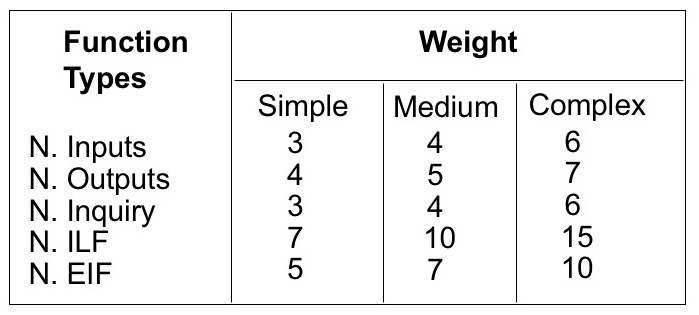
\includegraphics[width=0.8\textwidth]{tex-images/FPTable}
\label{fig:functionpoints}
\caption{Function Points values}
\end{figure}

\begin{table}
\begin{center}
\begin{tabular}{ccc}
\toprule
Function                        & Complexity   & FP Cost \\
\midrule
Login                           &   LOW   &   3   \\
Logout                        &   LOW   &   3   \\
Passenger signup               &   LOW   &   3   \\
Driver signup                  &   MEDIUM   &   4   \\
Require Taxi                  &   MEDIUM   &   4   \\
Reserve Taxi                  &   MEDIUM   &   4   \\
GPS reading                     &   LOW   &   3   \\
Modify or delete reservation   &   LOW   &   3   \\
Driver availability            &   LOW   &   3   \\
Driver accepting or declining   &   LOW   &   3   \\
\midrule
Subtotal                        &         &   33   \\
\bottomrule
\end{tabular}
\caption{Input functions}
\end{center}
\end{table}

%%%%%%%%%%%%%%%%%%%%%%%%%%%%%%%%%%%%%%%%

\begin{table}
\begin{center}
\begin{tabular}{ccc}
\toprule
Function                        & Complexity   & FP Cost \\
\midrule
Driver assignment notification   &   LOW   &   4   \\
Driver move elsewhere         &   HIGH   &   7   \\
Passenger request confirmation   &   HIGH   &   7   \\
Passenger reservation confirmation   &   MEDIUM   &   5   \\
Passenger res unavailable      &   MEDIUM   &   5   \\
\midrule
Subtotal                        &         &   28   \\
\bottomrule
\end{tabular}
\caption{Output functions}
\end{center}
\end{table}

%%%%%%%%%%%%%%%%%%%%%%%%%%%%%%%%%%%%%%%%

\begin{table}
\begin{center}
\begin{tabular}{ccc}
\toprule
Function                        & Complexity   & FP Cost \\
\midrule
See reservation history         &   LOW   &   3   \\
\midrule
Subtotal                        &         &   3   \\
\bottomrule
\end{tabular}
\caption{Inquiry functions}
\end{center}
\end{table}


\begin{table}
\begin{center}
\begin{tabular}{ccc}
\toprule
Function                           & Complexity   & FP Cost \\
\midrule
Passengers database               &   LOW   &   7   \\
Taxi and taxi driver database      &   LOW   &   7   \\
Requests database                  &   LOW   &   7   \\
City zones database               &   LOW   &   7   \\
\midrule
Subtotal                           &          &   28   \\
\bottomrule 
\end{tabular}
\caption{Internal Logic Files functions}
\end{center}
\end{table}

\subsection{Conclusions}
 By counting functional operations in the system and assigning them appropriate values, we obtain an Unadjusted Function Points (UFP) count. If we multiply this by the appropriate programming language scale factor, which equals to 46 for Java EE (according to \href{http://www.qsm.com/resources/function-point-languages-table}{this resource}), we obtain the Lines of Code (LOC) count for the project, thereby obtaining a size estimate.
\begin{center}
$ LOC = UFP \times 46 $
\end{center}
Function Point count, as it emerges from the analysis depicted in this section's tables, is:
\begin{center}
$ UFP = 33 + 28 + 3 + 28 = 125 $
\end{center}
And this finally gives us:
\begin{center}
$ LOC = 125 \times 46 = 5750$
\end{center}
This estimation on the source lines of code can then be used as input for other analysis methods, such as COCOMO II.

%%%%%%%%%%%%%%%%%%%%%%%%%%%%%%%%%%%%%%%%
%%%%%%%%%%%%%%%%%%%%%%%%%%%%%%%%%%%%%%%%

\section{COCOMO II analysis}
COCOMO II analysis uses two different sets of parameters: Scale and Cost Drivers. Definitions, tables and values are taken from the \href{http://csse.usc.edu/csse/research/COCOMOII/cocomo2000.0/CII_modelman2000.0.pdf}{COCOMO II Model Definition Manual}.

\subsection{Scale Drivers}

\begin{table}
\begin{center}
\begin{tabular}{ccc}
\toprule
Driver         &   Magnitude   &    Value \\
\midrule
Precedentness   &   VERY LOW   &   6.20   \\
Flexibility      &   NOMINAL   &   3.04   \\
Risk resolution      &   NOMINAL   &   4.24   \\
Team cohesion   &   HIGH   &   2.19   \\
Process maturity   &   NOMINAL   &   4.68   \\
\midrule
Total sum      &        &   20.35   \\
\bottomrule
\end{tabular}
\caption{COCOMO Scale drivers}
\end{center}
\end{table}

Precedentness relates to how familiar the type of project is to its developers, and this is being a first for us, it can only take the lowest value. Flexibility and Risk resolution have been rated to a medium value because of the didactic nature of this project -- as a toy example and not an actual real-life business application, we had much more freedom that what would have otherwise been. Team cohesion has been rated high thanks to our mutual understanding and a bit of history of working together. As for the Process maturity, it has been estimated through a rough application of a CMM-like classification, as suggested.

\subsection{Cost Drivers}

\begin{table}
\begin{center}
\begin{tabular}{ccc}
\toprule
Driver        				 &   Magnitude   	&    Value \\
\midrule
Required software reliability	 &   VERY LOW   	&    0.82 \\
Database size			 &   NOMINAL   	&    1.00 \\
Product complexity			 &   NOMINAL   	&    1.00 \\
Required reusability			 &   NOMINAL   	&    1.00 \\
Documentation match		 &   NOMINAL   	&    1.00 \\
Execution time constrain		 &   NOMINAL   	&    1.00 \\
Main storage constraint		 &   n/a   		&    n/a \\
Platform volatility			 &   LOW	   	&    0.87 \\
Analyst capability			 &   HIGH	   	&    0.85 \\
Programmer capability		 &   NOMINAL   	&    1.00 \\
Personnel continuity		 &   VERY HIGH   	&    0.81 \\
Application experience		 &   VERY LOW   	&    1.22 \\
Platform experience		 &   LOW 	  	&    1.09 \\
Language and tool experience	 &   LOW	   	&    1.09 \\
Usage of software tools		 &   NOMINAL   	&    1.00 \\
Multisite development		 &   EXTRA HIGH   	&    0.80 \\
Required development schedule	 &   NOMINAL   	&    1.00 \\
\midrule
Total product			 &   		  	&    0.57 \\
\bottomrule
\end{tabular}
\caption{COCOMO Cost drivers}
\end{center}
\end{table}

\begin{description}
\item[Required software reliability] The application does not manage important data at all, and even if a failure leads to a loss of service for some users, they lose a taxi ride at most;
\item[Database size] The real size of the databases is unknown, but they would be at most of medium size, and the estimated SLOC are in the thousands;
\item[Product complexity] The value was estimated as medium following the CPLEX rating scale;
\item[Required reusability] A modular structure is always good, but there is no need to overachiev;
\item[Documentation match to life-cycle needs] The documentation provided in other documents, and the requirement and design detailed, are neither too much nor too little work;
\item[Execution time constraint] The system does not need to satisfy narrow, real-time constraints, but it is still required to work with dates, hours and minutes and send messages appropriately, working within seconds (or tens of seconds) of the timestamp triggers, and moreover it must constantly monitor city-wide taxi coverage, reacting to changes and movements;
\item[Main storage constraint] In 2016 there is no such thing as a \emph{space constraint} for a project of this size -- the databases emplyed here are far smaller than what a typical business would have;
\item[Platform volatility] We can assume a very stable work situation without frequent innovations;
\item[Analyst capability] We put a lot of effort in defining requirements and design, and even if these have not been tested on the field (implementing properly), we believe them to be sound enough;
\item[Personnel continuity] In a real case in which we were developing this, we would surely be there from the beginning to the end of the process;
\item[Application experience] We never did anything of the sort (developing in Java EE, building a web app, and so on);
\item[Platform experience] While we have been studying the theoretical workings of the components (databases, user interfaces, etc) we never actually used them anywhere in practice;
\item[Language and tool experience] While we have been studying the theoretical workings of language and tools we never actually used them anywhere in practice;
\item[Usage of software tools] While not extensive, we do have knowledge of use of Integrated Development Enviroments, dependencies managers, collaborative effort trackers and version controllers;
\item[Multisite development] We worked together most of the time, in person, and communicated with today's means when needed;
\item[Required development schedule] We were always on time and the workload was always balanced, leading to no need to stretch or compress the schedule.
\end{description}

\subsection{Conclusions}
The Effort equation is as follow:
\begin{center}
$ E_f = A \times EAF \times KSLOC^e $
\end{center}
where \emph{A} is a standardized parameter equal to 2.94, \emph{EAF} is the product of the Cost Drivers, equal to 0.57, KSLOC is thousands of lines of code (estimated at 5.75 through Function Point analysis) and \emph{e} is another parameter calculated as:
\begin{center}
$ e = B + 0.01 \times \sum\nolimits_{SF_i \in SF(I)} $
\end{center}
where B is a standardized parameter equal to 0.91 and \emph{SF} is the set of the Scale Factors, whose sum is 20.35. This leads to:
\begin{center}
$ e = 0.91 + 0.01 \times 20.35 = 1.1135 $
\end{center}
which in turn entails:
\begin{center}
$ E_f = 2.94 \times 0.57 \times 5.75^{1.1135} = 11.75 $
\end{center}
which means a little less than a full person-year, or twelve person-months.

With Effort in hand, we may estimate Duration with the following:
\begin{center}
$ D_u = 3.67 \times {E_f}^d $
\end{center}
where \emph{d} is the schedule equation exponent, whose value is:
\begin{center}
$ d = D + 0.2 \times (e - B) $
\end{center}
where \emph{D} is a standardized parameter equal to 0.28 and \emph{e} and \emph{B} have been previusly defined. This leads to:
\begin{center}
$ d = 0.28 + 0.2 \times (1.1135 - 0.91) = 0.3207 $
\end{center}
so that we may obtain the final result for the Duration:
\begin{center}
$ D_u = 3.67 \times {11.75}^{0.3207} = 8.09 $
\end{center}

From this, we can finally extract the required number of people with the formula:
\begin{center}
$ N_p = \dfrac{E_f}{D_u} = \dfrac{11.75}{8.09} = 1.45 \approx 2 $
\end{center}